%%%%%%%%%%%%%%%%%%%%%%%%%%%%%%%%%%%%%%%%%%%%%%%%%%%%%%%%%%%%%%%%%%%%%%%%%%%%%%%%%%%%%
% Industrial implementations of RL
%
%
% 
%%%%%%%%%%%%%%%%%%%%%%%%%%%%%%%%%%%%%%%%%%%%%%%%%%%%%%%%%%%%%%%%%%%%%%%%%%%%%%%%%%%

This chapter starts with a literature review on the most famous RL applications in history.  Applications in this section have all been widely covered by the media and are well known amongst researchers and industrial practitioners alike.  Then, a review on RL applications catered towards the process control industry will be provided. Finally, this chapter is concluded with an impressive application of RL for power optimization. The main contribution of this chapter is the conducted literature view.

\section{Renowned triumphs}
The world witnessed, for the first time, artificial intelligence learning and playing games with a mere camera placed in front of the computer screen \cite{dqn1, dqn2}!  In this application, a general RL agent \textit{successfully} conquered various ATARI games using the camera images alone. However, such games are simple near-deterministic environments with sufficiently small state and action spaces, allowing even rules-based methods to be near-optimal (though previous algorithms did not \textit{learn} the games, nor can they play multiple games with the same algorithm). Although DQN showcased the power and generality of DQN, previous methods were already near-optimal in such simple environments. To conquer a task never done before by computers, Google DeepMind developed AlphaGo in 2016.  AlphaGo was an RL algorithm built to conquer Go, an ancient 2-player board game invented 3,000 years ago in China \cite{alphago1, alphago2}. Go is widely known as a near-impossible game for machines due to the insane dimensions of its state and action space (over $10^{170}$ possible states, a googol times larger than Chess), and the requirement to defeat opponents with stochastic strategies. State-of-the-art Go programs struggle against even amateur players; however, AlphaGo decisively defeated Ke Jie, the world's best Go player. The structure of AlphaGo employs \textit{value networks} to evaluate the board state. Then, \textit{policy networks} are used for optimal action selection.  During initial training, the agent used supervised learning to gain fundamental knowledge from amateur level play.  Afterwards, advanced strategies were developed by learning from expert level play.  After surpassing the experts, the agent continued to \textit{perfect} itself through conducting playing against itself, ultimately evolving into the world's best Go player in history \cite{alphago1, alphago2}. In terms of real world applications, these experiments demonstrate the potential of RL to identify new techniques and insights to advance modern engineering beyond what is already known.














\section{Simulated RL applications}

















\section{Google's success story}
A world-changing implementation of RL was demonstrated by Google when a RL agent\footnote{Google DeepMind did not explicitly state the technology used to achieve the savings, only machine learning. However, DeepMind is a company that focuses on reinforcement learning approaches and there were many mentions of creating a general algorithm for all the data centers in the article; therefore, it was assumed reinforcement learning was used. More specifically, meta-RL was most likely used due to the construction of many simulators and the agent's adaptation speed.} showed the capabilities to autonomously controlling a \textit{live} data center, reducing electricity usage by up to 40\%. This also indirectly reduced the carbon footprint of all individuals using Google's services, which encompasses a large part of the world. Google's data centers generate enormous amounts of heat through powering services such as Google Search, Gmail, and YouTube. Hence, the data centers' primary energy usage is for cooling. Cooling industrial processes are accomplished by equipment such as heat exchangers, pumps, and cooling towers---even at Google.  Modelling such a complex, non-linear systems poses several difficulties, rendering traditional methods ineffective \cite{google_data1}:
\begin{enumerate}
    \item Complex, high-dimensional environment with uncountable non-linear interactions rendering modern system identification methods infeasible. Additionally, experienced human operators simply cannot comprehend the countless interactions.
    \item Highly dynamic internal and external building conditions (such as ambient temperature, server load, etc.) rendering rules- and non-adaptive methods intractable.
    \item All data centers have unique layouts and set-ups.  This non-consistency demands custom-tuned models for each individual data center, assuming traditional approaches were used; however, such a dilemma could be adequately overcame through artificial general intelligence where one algorithm can learn many different scenarios.
\end{enumerate}
To overcome these difficulties, DeepMind researchers first identified neural network models corresponding to different operating conditions by leveraging historical operating data from different data centers.  The inputs to the neural network models were sensor information such as temperature, pump speeds, ambient temperature, etc. The model output was the power usage effectiveness (PUE) given by:
\begin{equation}
    PUE = \frac{\text{Total building energy usage}}{\text{IT energy usage}}
    \label{eq:pue}
\end{equation}
Here, the neural networks were used as training simulators for the data centers. RL was applied on said simulators to learn a control policy to minimize the PUE. Different agents were trained on different data centers, during different operating conditions. When implemented, the ideal agent would be picked based on the current operating condition. Initially, the control actions provided by the agent were only recommendations.  The PUE with and without implementing the agent's recommendations is shown in Figure \ref{fig:google_data_center}.

\begin{figure}[H]
    \centering
    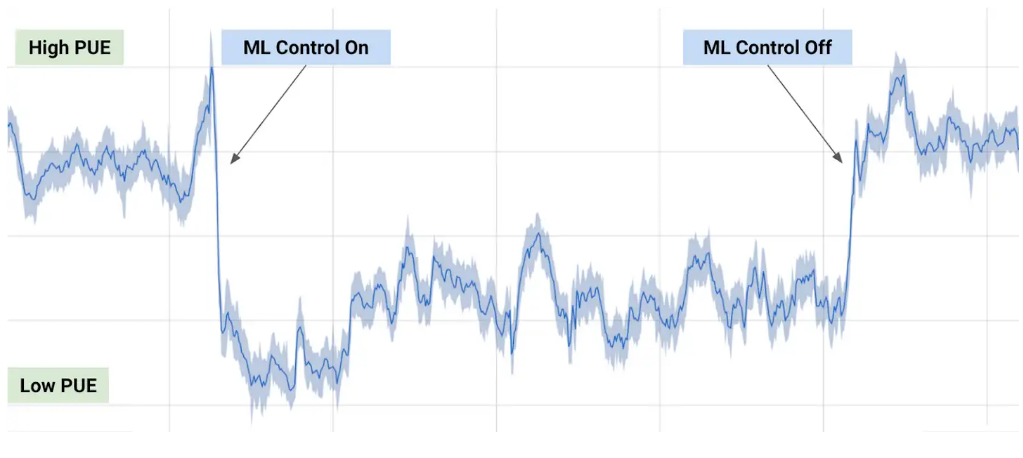
\includegraphics[width=0.7\textwidth]{images/ch5/google_data_center.jpeg}
    \caption{Power usage effectiveness with and without ML control.  Original figure from \cite{google_data1}.}
    \label{fig:google_data_center}
\end{figure}

By 2018, the agent was given full access to the data center control system after safety constraints were added. 

As a summary, the RL agents sample measurements from the sensors in each data center every five minutes and outputs the optimal control actions that satisfy a robust set of safety constraints \cite{google_data2}. The local control operators then verify the provided inputs to ensure that the system will remain within constraint boundaries. In the first few months, the agent consistently reduced electricity consumption by an average of 30\% and is expected to improve as it continues to learn. In the end, the agent reached an optimal policy that resulted in the lowest PUE ever seen, far surpassing human operation---an event only achievable through RL.
